% !TeX spellcheck = en_US
\section{Architecture of the Quality Assessment Framework}
\label{sec:553_Architecture}
In the proposed scenario, a scalable and adaptive quality assessment is a precondition for quality-aware content adaptation.
Novel aspects of this proposed assessment are the respect for varying application requirements, adaptive algorithms, and scalability by leveraging the resources of the mobile devices.

\emph{Varying application requirements} are addressed as multimedia applications (e.g., pursuing video composition) can specify the minimal precision required for an assessment and the maximum runtime until it is completed.

Recording degradations have not yet been analyzed by accurate, objective quality assessment algorithms.
Novel recording quality assessment algorithms are proposed, which offer high precision at a low runtime.
Proposed algorithms can \emph{adapt} between the signals to be analyzed to achieve given time and precision requirements.
Algorithms that can adapt between signals are presented in Figure~\ref{fig:553_architecture} as \emph{hybrid algorithms}.

\emph{Scalability} is achieved by selecting an appropriate algorithm that complies with the given requirements and dynamically places it on a node in the entire system to efficiently leverage the available resources.
As a result, this chapter proposes an algorithm selection and placement.

\begin{figure}[!htb]
\centering
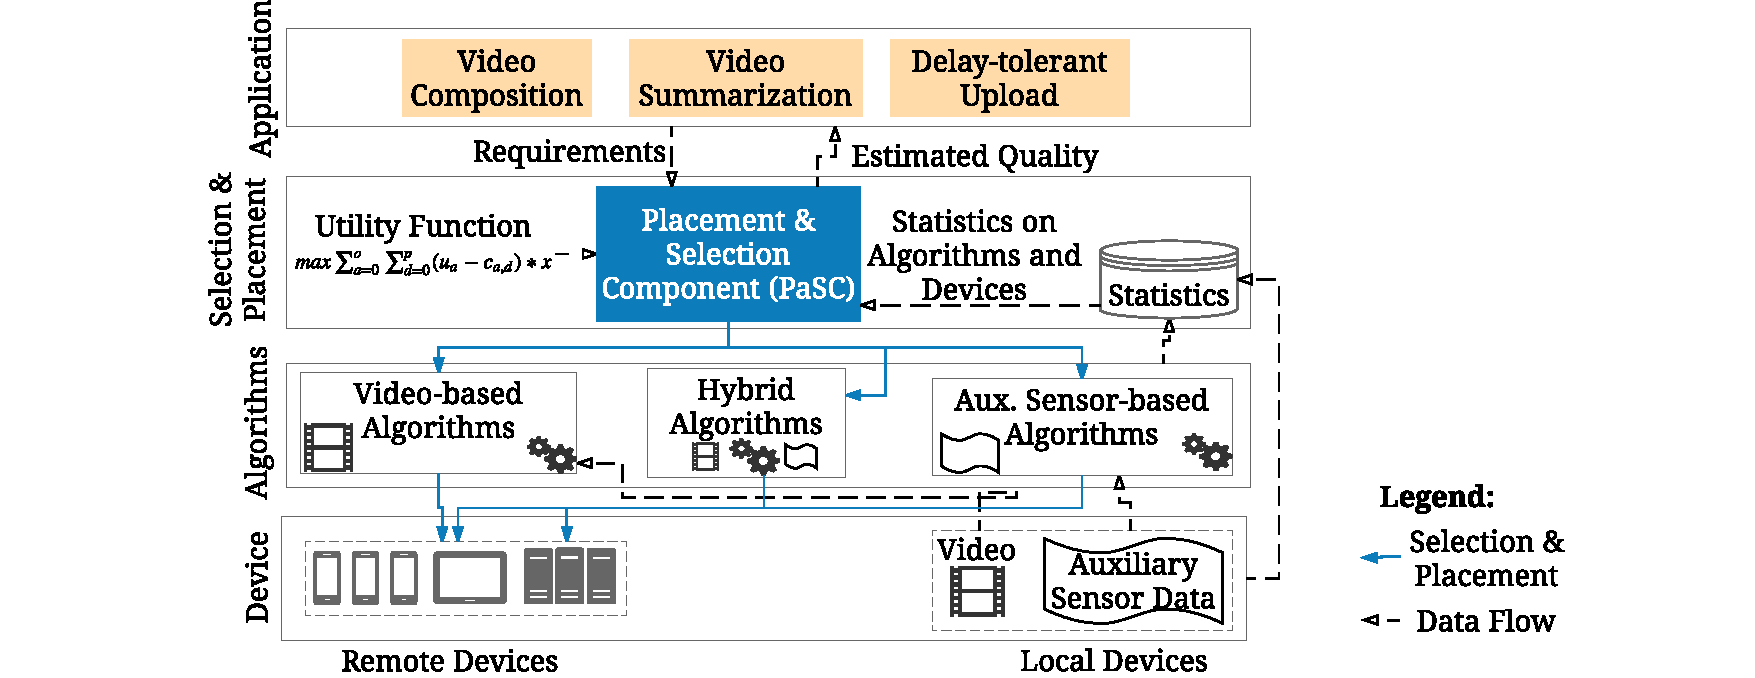
\includegraphics[width=\linewidth]{./gfx/550_QA/VIDEO_QUALITY_ARCHITECTURE}
\caption{Architecture of the scalable, objective quality assessment}
\label{fig:553_architecture}
\end{figure}
As depicted in Figure~\ref{fig:553_architecture}, a system architecture is proposed to achieve scalability and awareness of application requirements for obtaining an objective quality assessment.
An application requires two modifications to integrate the scalable video quality assessment.
First, the application needs to specify its requirements for the quality assessment by setting a deadline, when the execution needs to be completed, and the desired precision of the algorithm. 
Second, the application must be able to receive the quality assessment result.

The \ac{PaSC} is responsible for the selection of a quality assessment algorithm and its placement on a device.
All quality assessment algorithms are designed to run on different devices (i.e., see "Device" layer in Figure~\ref{fig:553_architecture}\footnote{The implementation allows the execution of Java-based systems, i.e., Android smartphones and tablets, too. Performance metrics are gathered on a realization of the algorithms in C.}).
Whereas a camera, microphones, and other necessary sensors are used on a local device, other devices that run the proposed system are leveraged for algorithm execution. Algorithms are classified into classical video-based and auxiliary sensor-based ones. This classification is applied to algorithms proposed in earlier work (see Section~\ref{sec:210_ojective_quality}) and the novel algorithms, which are presented in this thesis.

The \ac{PaSC} also receives the quality assessment result and transmits it to the application. 
Except for the central repository for statistics, the component including the algorithm definitions is available on each device. 
As intended, it offers a distributed usage of the system. 
As depicted in Figure~\ref{fig:553_architecture}, the \ac{PaSC} uses runtime statistics from a central repository.
This repository keeps track of algorithm execution times and stores device statistics on delay, energy, \ac{CPU} and memory utilization.

The monitoring of system characteristics happens in an event-driven manner. 
As soon as the monitored device statistics change, the device pushes updates to the central repository.